% Options for packages loaded elsewhere
\PassOptionsToPackage{unicode}{hyperref}
\PassOptionsToPackage{hyphens}{url}
%
\documentclass[
]{article}
\title{A Bayesian hierarchical mixture cure modelling (MCM) framework
for the joint utilization of progression free survival (PFS) and overall
survival (OS) in estimating long-term survivorship (LTS) rates in
previously untreated metastatic melanoma: A case study from
CheckMate-067 trial}
\author{Nathan Green, Gianluca Baio, UCL}
\date{07 December, 2021}

\usepackage{amsmath,amssymb}
\usepackage{lmodern}
\usepackage{iftex}
\ifPDFTeX
  \usepackage[T1]{fontenc}
  \usepackage[utf8]{inputenc}
  \usepackage{textcomp} % provide euro and other symbols
\else % if luatex or xetex
  \usepackage{unicode-math}
  \defaultfontfeatures{Scale=MatchLowercase}
  \defaultfontfeatures[\rmfamily]{Ligatures=TeX,Scale=1}
\fi
% Use upquote if available, for straight quotes in verbatim environments
\IfFileExists{upquote.sty}{\usepackage{upquote}}{}
\IfFileExists{microtype.sty}{% use microtype if available
  \usepackage[]{microtype}
  \UseMicrotypeSet[protrusion]{basicmath} % disable protrusion for tt fonts
}{}
\makeatletter
\@ifundefined{KOMAClassName}{% if non-KOMA class
  \IfFileExists{parskip.sty}{%
    \usepackage{parskip}
  }{% else
    \setlength{\parindent}{0pt}
    \setlength{\parskip}{6pt plus 2pt minus 1pt}}
}{% if KOMA class
  \KOMAoptions{parskip=half}}
\makeatother
\usepackage{xcolor}
\IfFileExists{xurl.sty}{\usepackage{xurl}}{} % add URL line breaks if available
\IfFileExists{bookmark.sty}{\usepackage{bookmark}}{\usepackage{hyperref}}
\hypersetup{
  pdftitle={A Bayesian hierarchical mixture cure modelling (MCM) framework for the joint utilization of progression free survival (PFS) and overall survival (OS) in estimating long-term survivorship (LTS) rates in previously untreated metastatic melanoma: A case study from CheckMate-067 trial},
  pdfauthor={Nathan Green, Gianluca Baio, UCL},
  hidelinks,
  pdfcreator={LaTeX via pandoc}}
\urlstyle{same} % disable monospaced font for URLs
\usepackage[margin=1in]{geometry}
\usepackage{longtable,booktabs,array}
\usepackage{calc} % for calculating minipage widths
% Correct order of tables after \paragraph or \subparagraph
\usepackage{etoolbox}
\makeatletter
\patchcmd\longtable{\par}{\if@noskipsec\mbox{}\fi\par}{}{}
\makeatother
% Allow footnotes in longtable head/foot
\IfFileExists{footnotehyper.sty}{\usepackage{footnotehyper}}{\usepackage{footnote}}
\makesavenoteenv{longtable}
\usepackage{graphicx}
\makeatletter
\def\maxwidth{\ifdim\Gin@nat@width>\linewidth\linewidth\else\Gin@nat@width\fi}
\def\maxheight{\ifdim\Gin@nat@height>\textheight\textheight\else\Gin@nat@height\fi}
\makeatother
% Scale images if necessary, so that they will not overflow the page
% margins by default, and it is still possible to overwrite the defaults
% using explicit options in \includegraphics[width, height, ...]{}
\setkeys{Gin}{width=\maxwidth,height=\maxheight,keepaspectratio}
% Set default figure placement to htbp
\makeatletter
\def\fps@figure{htbp}
\makeatother
\setlength{\emergencystretch}{3em} % prevent overfull lines
\providecommand{\tightlist}{%
  \setlength{\itemsep}{0pt}\setlength{\parskip}{0pt}}
\setcounter{secnumdepth}{-\maxdimen} % remove section numbering
\newlength{\cslhangindent}
\setlength{\cslhangindent}{1.5em}
\newlength{\csllabelwidth}
\setlength{\csllabelwidth}{3em}
\newlength{\cslentryspacingunit} % times entry-spacing
\setlength{\cslentryspacingunit}{\parskip}
\newenvironment{CSLReferences}[2] % #1 hanging-ident, #2 entry spacing
 {% don't indent paragraphs
  \setlength{\parindent}{0pt}
  % turn on hanging indent if param 1 is 1
  \ifodd #1
  \let\oldpar\par
  \def\par{\hangindent=\cslhangindent\oldpar}
  \fi
  % set entry spacing
  \setlength{\parskip}{#2\cslentryspacingunit}
 }%
 {}
\usepackage{calc}
\newcommand{\CSLBlock}[1]{#1\hfill\break}
\newcommand{\CSLLeftMargin}[1]{\parbox[t]{\csllabelwidth}{#1}}
\newcommand{\CSLRightInline}[1]{\parbox[t]{\linewidth - \csllabelwidth}{#1}\break}
\newcommand{\CSLIndent}[1]{\hspace{\cslhangindent}#1}
\ifLuaTeX
  \usepackage{selnolig}  % disable illegal ligatures
\fi

\begin{document}
\maketitle

\hypertarget{executive-summary}{%
\subsubsection{Executive summary}\label{executive-summary}}

In this project we formulate and demonstrate the application of a
Bayesian mixture cure model (MCM) using the Checkmate 067 study dataset
for a range of survival distributions. Analogous results to those
created previously for the frequentist MCM approach are produced and we
extend the Bayesian MCM to incorporate additional structure. This
includes modelling the cure fractions separately for OS and PFS (as in
the frequentist approach) and by joining the overall survival (OS) and
progression-free survival (PFS) models using a hierarchical (multilevel)
structure on the cure fraction. We show that the Exponential and in
particular the log-logistic OS and PFS Bayesian MCMs perform reasonably
well for the Checkmate 067 data. We also perform a sensitivity analysis
by increasing the background hazard rate via a hazard ratio adjustment,
representing a study population with a higher mortality rate than the
general population. The real benefit of this approach, not full explored
in this analysis, may be with other dataset where there is relatively
short follow-up or small sample sizes. The associated R code for this
work, held in a private on-line repository, has been written for re-use
and generalisability to other problems.

\hypertarget{background}{%
\subsection{Background}\label{background}}

Immuno-oncologic (IO) studies for melanoma therapies, such as
\emph{ipilimumab} (\texttt{ipi}), \emph{nivolumab} (\texttt{nivo}), and
the \emph{nivolumab} with \emph{ipilimumab} (\texttt{nivo\ +\ ipi})
combination, have indicated that survival curves ``plateau'' (a
considerable proportion of patients are ``long-term survivors (LTS)'').
Emergent survival plateaus in a survival model may be represented within
a mixture cure model (MCM). Usually event times, e.g.~for PFS and OS,
are modelled separately but this may lead to a clinically unintuitive
dichotomy between proportions of long-term survivors. It is not always
possible to model PFS and OS jointly because we often have to rely on
synthetic data from digitized curves, which make it impossible to
retrieve the underlying correlation between the two outcomes. But if we
have access to trial data, like in the Checkmate 067 trail case, we
should make the most of it.

Cure models are a special type of survival analysis where this ``cure
fraction'' (the underlying proportion of responders to
treatment/long-term survivors) is accounted for. Cure models estimate
the cure fraction, in addition to a parametric survival function for
patients that are not cured. The mortality risk in the cured patients is
informed by a background mortality rate. The population that is not
cured is subject both to background mortality and to additional
mortality from their cancer, estimated using a parametric survival
model. A mixture cure model (MCM) (Amico and Van Keilegom (2018)) is a
type of cure model where survival is modelled as a mixture of two groups
of patients: those who are cured and those who are not (and who
therefore remain at risk). The survival for a population with a cure
fraction can be written as follows:

\begin{align}
\tag{*}
S(t, x) = S^*(t, x)[\pi(x) + (1 − \pi(x))S_u(t, x)],
\end{align}

where \(S(t, x)\) denotes the survival at time \(t\), \(S^*(t, x)\)
denotes the background mortality at time \(t\) conditional on covariates
\(x\), \(\pi(x)\) denotes the probability of being cured conditional on
covariates \(x\), and \(S_u(t, x)\) denotes the event (progression or
mortality) due to cancer at time \(t\) conditional on covariates \(x\).
For PFS, the survival is composed of either progressing to a disease
state or death.

\hypertarget{aims}{%
\subsection{Aims}\label{aims}}

The aims of the the analysis in this document are as follows:

\begin{itemize}
\tightlist
\item
  Demonstrate the application of a Bayesian mixture cure model using the
  Checkmate 067 study dataset and the Exponential distribution for event
  times.
\item
  Produce analogous results to those created previously for the
  frequentist approach.
\item
  Extend the Bayesian model to incorporate additional structure
  including a hierarchical cure fraction.
\end{itemize}

This analysis has been carried-out using the Stan inference engine
(Carpenter et al. (2017)) called from R on a Windows PC. The packaged
code can be downloaded from a private GitHub repository with permission
from the package authors at
\url{https://github.com/StatisticsHealthEconomics/rstanbmcm}. See the
\emph{How to use rstanbmcm} vignette for an introduction to how to use
the package.

\hypertarget{likelihood}{%
\subsection{Likelihood}\label{likelihood}}

Let \(T_i\) be the non-negative random variable denoting the survival
time of patient \(i\) with covariate vector \(\boldsymbol{x}_i\).

In the simplest case we can assume that the cure fraction is the same
for the whole population i.e.~\(\pi\) is fixed. Further, we can assume
the \(\pi\) models the relationship between \(\boldsymbol{x}_i\) and the
probability of being cured. E.g. using a logistic-linear model

\[
\pi(\boldsymbol{x}_i | \boldsymbol{\beta}) = 1/[1 + \exp(-\boldsymbol{x}_i^T \boldsymbol{\beta})].
\]

The likelihood of the standard survival is

\[
L = \prod_i S(t_i | \boldsymbol{x}_i) h(t_i | \boldsymbol{x}_i)^{\delta_i}
\]

Log-likelihood is therefore \[
\mathcal{l} = \sum_i \log(S(t_i | \boldsymbol{x}_i)) + \delta_i \log(h(t_i | \boldsymbol{x}_i))
\]

Plugging this directly into the mixture cure equation in (*) gives

\[
\mathcal{l}(\pi | \boldsymbol{\delta}, \boldsymbol{x}) =
 \sum_i \log(S^*(t_i | \boldsymbol{x}_i) h^*(t_i | \boldsymbol{x}_i)^{\delta_i}[\pi(x) +
   (1 − \pi(x)) S_u(t_i | \boldsymbol{x}_i) h_u(t_i | \boldsymbol{x}_i)^{\delta_i}])
\]

If we assume that the cured component is the Exponential survival model
then the non-cured component can be thought of in similar terms to the
cumulative incidence function. That is, the probability of an event is
the combined probability of surviving both events (e.g.~for OS,
all-cause and cancer mortality) and then experiencing either i.e.
dropping the \(S\) dependencies for brevity

\begin{equation}
\tag{**}
S^* S_u (h^*)^{\delta} + S^* S_u (h_u)^{\delta} = S^* S_u (h^* + h_u)^{\delta}
\end{equation}

\hypertarget{bayesian-formulation}{%
\subsection{Bayesian formulation}\label{bayesian-formulation}}

In a Bayesian approach to modelling (McElreath (2018)), all quantities
that are subject to uncertainty are modelled using probability
distributions. This applies to observed data (e.g.~time to PFS for a
given individual), that are subject to sampling variability, as well as
to unobservable parameters (e.g.~the coefficient quantifying the impact
of age or sex over the average survival curve). In this latter case,
probability distributions are used to model the epistemic uncertainty
(e.g.~the fact that we do not know for certain what the ``true''
underlying value of the model parameter is). In addition, we may model
as yet unobserved (but potentially observable) quantities using a
suitable probability model. For example, we could consider the
extrapolated part of the survival curve as subject to uncertainty due to
the current sampling process giving rise to the data that are actually
observed, as well as the uncertainty on the underlying data generating
process.

We can mix different sources of evidence to form our ``prior''
distributions, which are used to describe the state of science on the
model parameters. These are then combined with any observed data to form
an updated level of knowledge. This process is particularly relevant in
the case at hand, when data can only inform about limited aspects of the
overall underlying reality. For this reason, it is important to a)
include information/evidence available in the form of external data
and/or expert opinion; b) extract the most information possible from the
available data (e.g.~by formally trying to model the correlation between
the PFS and the OS data to borrow strength from the more mature set of
observations).

A built-in advantage of the Bayesian procedure is that uncertainty is
directly and formally propagated to an economic model; the main output
from the statistical analysis (the extrapolated survival curve) are
produced by default as based on a full posterior distribution. From
this, we can easily derive a ``base case'' (e.g.~taking the mean value)
but without the need for further tools (such as bootstrap) we already
have a full characterisation of the underlying uncertainty that can be
used in the process of probabilistic sensitivity analysis. We can
moreover add information in the priors to ensure that the extrapolation
beyond the observed data is realistic and consistent with the clinical
expertise (e.g.~by ``anchoring'' the extrapolated survival curve to be
probabilistically below the curves for the healthy population, or by
ensuring that OS behaves in a way to respect some agreed level of
similarity, or correlation, to PFS).

\hypertarget{posterior-equation}{%
\paragraph{Posterior equation}\label{posterior-equation}}

Using the likelihood function defined above and prior distributions on
uncertain parameters, we can specify the posterior distribution.
Defining \(g_2\) as the prior distribution for the coefficients of the
uncured fraction \(\beta^u\) and \(g_3\) as the prior distribution for
the coefficients of the cured fraction \(\beta^*\), then the general
form of the posterior distribution can be written as follows.

\[
p(\pi, \boldsymbol{\beta^u}, \boldsymbol{\beta^*} | \boldsymbol{\delta}, \boldsymbol{x}) \propto
L(\pi, \boldsymbol{\beta^u}, \boldsymbol{\beta^*} | \boldsymbol{\delta}, \boldsymbol{x}) f(\pi) g_2(\boldsymbol{\beta^u}) g_3(\boldsymbol{\beta^*})
\]

assuming that the cure fraction is independent of the covariates.

\hypertarget{cure-fraction}{%
\subsubsection{Cure fraction}\label{cure-fraction}}

There are two obvious ways to represent the uncertainty about the cure
fraction in the model.

The first is to specify the cure fraction directly using a
\(\pi \sim Beta(a_{cf}, b_{cf})\) prior, most uninformative as a uniform
\(Beta(1,1)\). The parameters can be obtained via transformation of mean
and standard deviation to allow a more natural scale for elicitation.

Alternatively, we may specify the uncertainty on the real line with a
Normal distribution and then transform to the probability scale.

A further consideration is how to represent the cure fraction so to
share information between the OS and PFS data. We will investigate 3
alternatives.

\begin{itemize}
\tightlist
\item
  \emph{Pooled}: Assume that the cure fraction is the same for OS and
  PFS i.e.~\(\pi_{os} = \pi_{os} = \pi\) where \[
  logit(\pi) \sim N(\mu_{cf}, \sigma_{cf}^2), \;\;
  \]
\item
  \emph{Separate}: Model each independently. \[
  logit(\pi_{os}) \sim N(\mu_{cfos}, \sigma_{cfos}^2), \;\;  
  logit(\pi_{pfs}) \sim N(\mu_{cfpfs}, \sigma_{cfpfs}^2)  
  \]
\item
  \emph{Hierarchical}: Assume exchangeability between OS and PFS\[
  \pi \sim N(\mu_{cf}, \sigma_{cf}^2), \;\;  
  logit(\pi_{os}) \sim N(\pi, \sigma_{cfos}^2), \;\;  
  logit(\pi_{pfs}) \sim N(\pi, \sigma_{cfpfs}^2)  
  \]
\end{itemize}

Below is an example DAG for the hierarchical cure fraction without a
joint time to event component. Notice that even without the direct
relationship between PFS and OS there is still an indirect influence via
\(\pi\).

\begin{figure}

{\centering 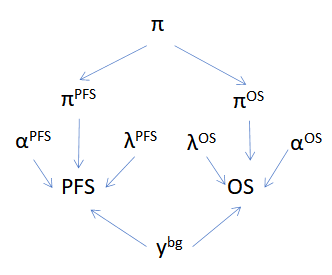
\includegraphics[width=0.4\linewidth]{hierarchical_DAG} 

}

\caption{\label{fig:hier_dag} Hierarchical cure fraction DAG.}\label{fig:unnamed-chunk-2}
\end{figure}

\hypertarget{background-survival}{%
\subsection{Background survival}\label{background-survival}}

The previous frequentist analysis used the World Health Organization
(WHO) life tables by country for the latest year available of 2016 (WHO
(2020)) to inform the background mortality rate (baseline hazard). These
baseline hazards are the expected mortality rate for each patient at the
age at which they experience the event. The mortality data are age- and
gender adjusted, thus providing a granular account of the different
patient profiles in the trial. The WHO reports conditional probabilities
of death in 5-year intervals until age 85. A constant annual mortality
rate is reported for individuals over 85. They assumed that the maximum
age is 100 years.

In a Bayesian analysis there are alternative ways in which we could
model the background mortality.

For this work we shall use WHO hazard point estimates as known. We could
consider the WHO estimates to provide sufficiently accurate estimates
given the sample size and so incorporating uncertainty is not necessary.
This also forces consistency across fits. Denote the WHO estimates for
individual \(i\) as \(\hat{f}_i, \hat{S}_i, \hat{h}_i\) for the density,
survival and hazard respectively.

This gives the likelihood

\[
L(\pi | \boldsymbol{\delta}, \boldsymbol{x}, \hat{S}, \hat{h}) =
\sum_i \hat{S}_i \hat{h}_i^{\delta_i} \left[ \pi(x) + (1 - \pi(x)) S_{u, i} h_{u , i}^{\delta_i} \right]
\]

\hypertarget{model-goodness-of-fit}{%
\subsection{Model goodness-of-fit}\label{model-goodness-of-fit}}

Model fit was determined using the leave-one-out (LOO) cross validation
statistics using WAIC (Vehtari, Gelman, and Gabry (2017)). A small
statistic is preferable.

\hypertarget{variance-partition-coefficient-vpc}{%
\subsection{Variance partition coefficient
(VPC)}\label{variance-partition-coefficient-vpc}}

The variance partition coefficient (VPC) is defined as
\(\sigma_{global}^2/ (\sigma_{global}^2 + \sigma_{e}^2)\) where
\(e = PFS\) or \(OS\). This indicates what proportion of the total
variance is attributable to variation within-groups, or how much is
found between-groups.

\hypertarget{results}{%
\subsection{Results}\label{results}}

We fit the separate and exchangeable cure fraction models to the study
data and produced the posterior survival curves below.

For each model and treatment we produce the expected survival curves
with 95\% Credible Intervals (CrI). The OS curves are to the left-hand
side and PFS curves to the right-hand side. Background mortality (i.e.
cured patients) is indicated by the red line. Non-cured patients
survival curves are shown in dark green and blue for OS and PFS
respectively. Light green and magenta are the total sample. The black
line is the Kaplan-Meier curve for the observed data. Note that these
plots are for an average individual, e.g.~at average age, and so we
would not expect them to perfectly match the sample data Kaplan-Meier.

\hypertarget{separate-survival-models-for-os-and-pfs}{%
\subsubsection{Separate survival models for OS and
PFS}\label{separate-survival-models-for-os-and-pfs}}

Figure \ref{fig:S_separate} shows posterior survival curves for the
Exponential, log-logistic, Gompertz, Weibull and log-Normal models when
the OS and PFS models are fitted separately.

\begin{figure}

{\centering 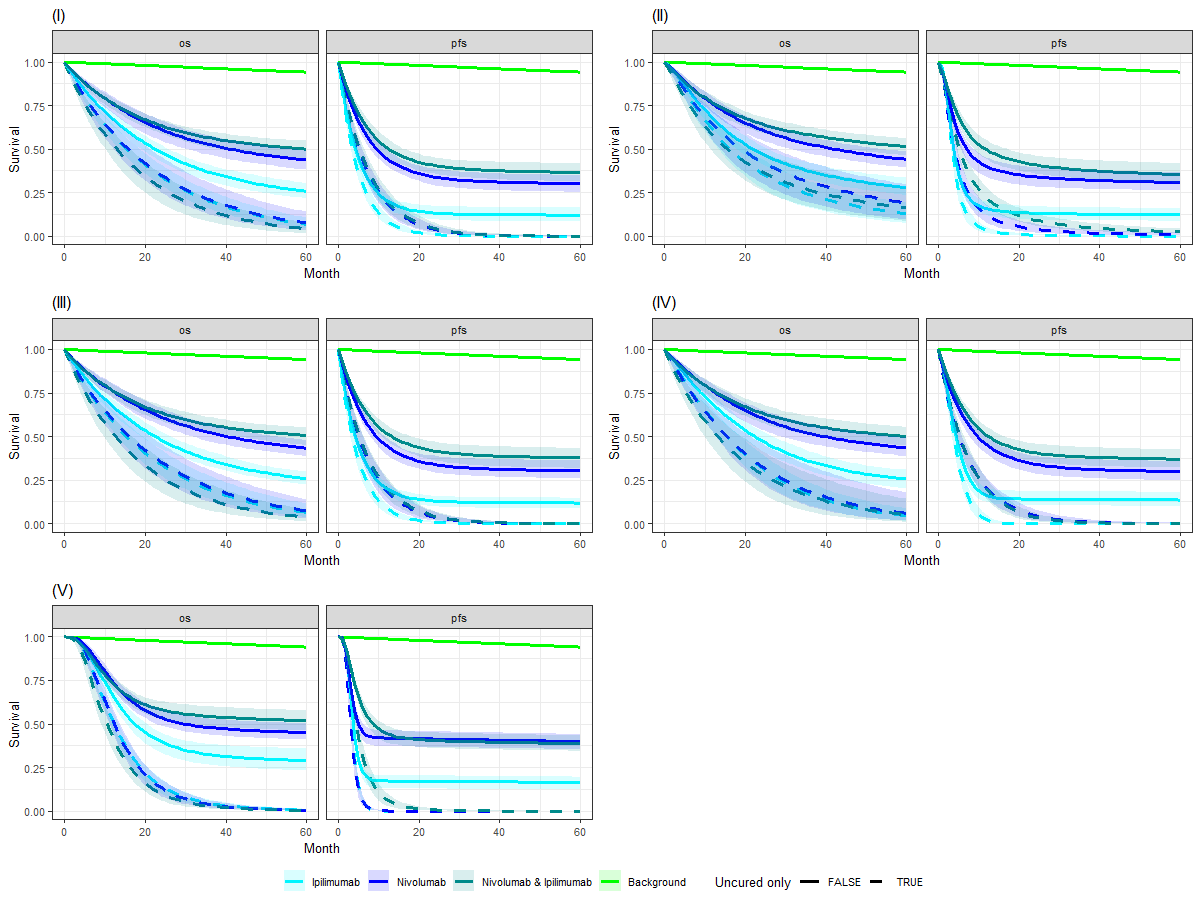
\includegraphics[width=15cm,height=40cm]{../plots/plot_S_samepair_grid_cf_separate_diffuncured} 

}

\caption{\label{fig:S_separate}Posterior survival curves for the mixture cure model for separate OS and PFS models and $ipilimumab$, $nivolumab$ and a combination treatment arm. The green line is cured background. Uncured distributions are I) Exponential  II) Log-logistic III) Gompertz IV) Weibull V) Log-Normal.}\label{fig:unnamed-chunk-3}
\end{figure}

Figure \ref{fig:forest_separate} shows the forest plots of cure fraction
posterior distributions.

\begin{figure}

{\centering 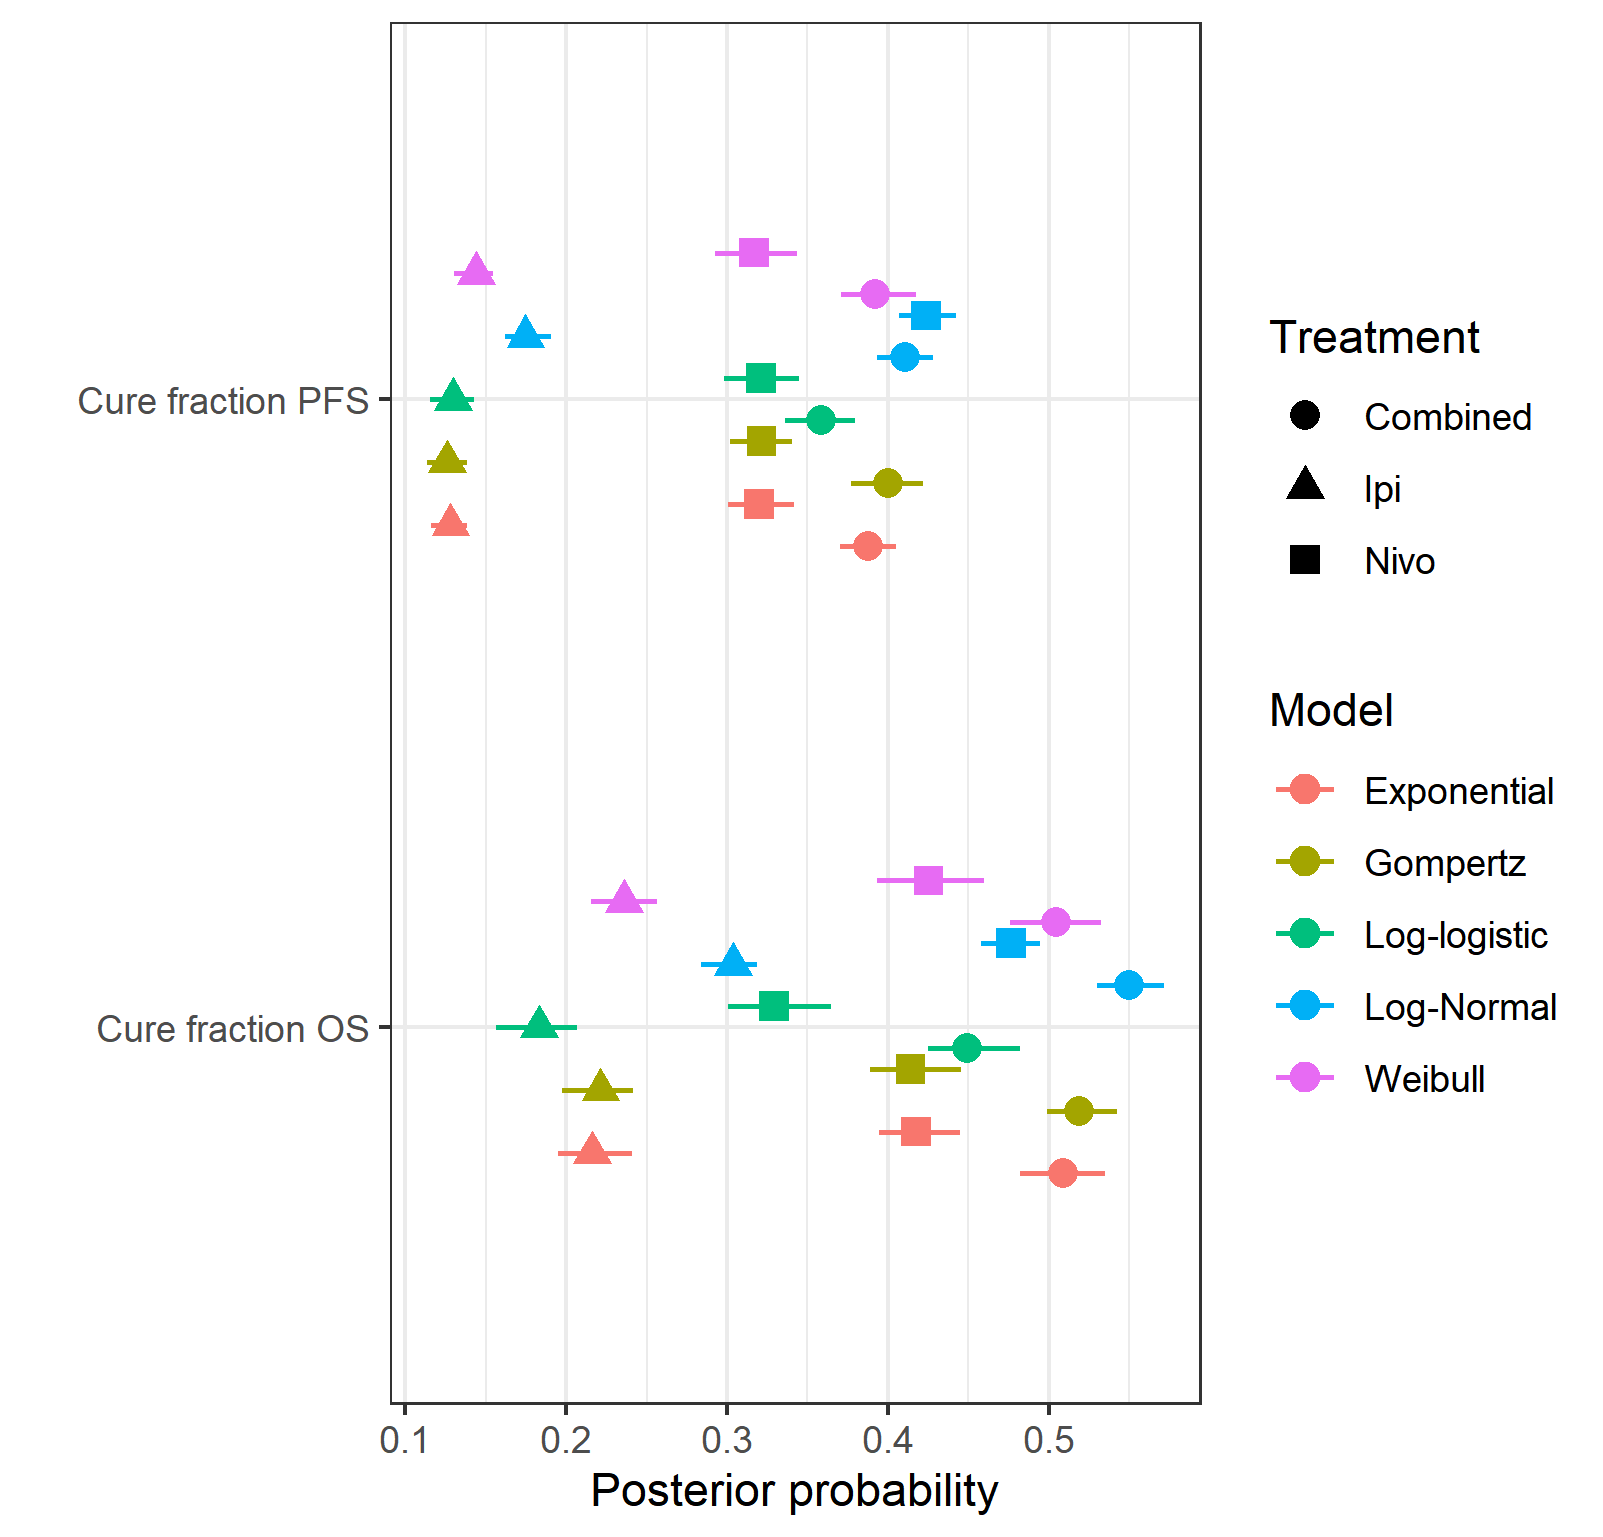
\includegraphics[width=0.6\linewidth]{../plots/cf separate_bg_fixed_forest_plot} 

}

\caption{\label{fig:forest_separate}Forest plot of cure fraction posterior distributions for separate OS and PFS models .}\label{fig:unnamed-chunk-4}
\end{figure}

Table 1 gives values for these posterior cure fractions.

\begin{longtable}[]{@{}
  >{\raggedleft\arraybackslash}p{(\columnwidth - 10\tabcolsep) * \real{0.03}}
  >{\raggedright\arraybackslash}p{(\columnwidth - 10\tabcolsep) * \real{0.13}}
  >{\raggedright\arraybackslash}p{(\columnwidth - 10\tabcolsep) * \real{0.13}}
  >{\raggedright\arraybackslash}p{(\columnwidth - 10\tabcolsep) * \real{0.23}}
  >{\raggedright\arraybackslash}p{(\columnwidth - 10\tabcolsep) * \real{0.23}}
  >{\raggedright\arraybackslash}p{(\columnwidth - 10\tabcolsep) * \real{0.23}}@{}}
\caption{Posterior cure fractions for separate model.}\tabularnewline
\toprule
\begin{minipage}[b]{\linewidth}\raggedleft
ID
\end{minipage} & \begin{minipage}[b]{\linewidth}\raggedright
OS distn
\end{minipage} & \begin{minipage}[b]{\linewidth}\raggedright
PFS distn
\end{minipage} & \begin{minipage}[b]{\linewidth}\raggedright
Treatment
\end{minipage} & \begin{minipage}[b]{\linewidth}\raggedright
\(cf_{OS}\) (CrI)
\end{minipage} & \begin{minipage}[b]{\linewidth}\raggedright
\(cf_{PFS}\) (CrI)
\end{minipage} \\
\midrule
\endfirsthead
\toprule
\begin{minipage}[b]{\linewidth}\raggedleft
ID
\end{minipage} & \begin{minipage}[b]{\linewidth}\raggedright
OS distn
\end{minipage} & \begin{minipage}[b]{\linewidth}\raggedright
PFS distn
\end{minipage} & \begin{minipage}[b]{\linewidth}\raggedright
Treatment
\end{minipage} & \begin{minipage}[b]{\linewidth}\raggedright
\(cf_{OS}\) (CrI)
\end{minipage} & \begin{minipage}[b]{\linewidth}\raggedright
\(cf_{PFS}\) (CrI)
\end{minipage} \\
\midrule
\endhead
1 & exp & exp & Ipilimumab & 0.216 (0.16, 0.271) & 0.128 (0.089,
0.173) \\
2 & exp & exp & Nivolumab & 0.417 (0.335, 0.482) & 0.32 (0.268, 0.37) \\
3 & exp & exp & Nivolumab+ipilimumab & 0.509 (0.43, 0.573) & 0.387
(0.332, 0.441) \\
4 & gompertz & gompertz & Ipilimumab & 0.221 (0.176, 0.282) & 0.126
(0.092, 0.156) \\
5 & gompertz & gompertz & Nivolumab & 0.414 (0.352, 0.477) & 0.321
(0.274, 0.383) \\
6 & gompertz & gompertz & Nivolumab+ipilimumab & 0.519 (0.444, 0.573) &
0.4 (0.338, 0.458) \\
7 & loglogistic & loglogistic & Ipilimumab & 0.183 (0.11, 0.265) & 0.13
(0.091, 0.168) \\
8 & loglogistic & loglogistic & Nivolumab & 0.329 (0.217, 0.423) & 0.321
(0.267, 0.381) \\
9 & loglogistic & loglogistic & Nivolumab+ipilimumab & 0.449 (0.349,
0.524) & 0.359 (0.308, 0.427) \\
10 & lognormal & lognormal & Ipilimumab & 0.304 (0.241, 0.378) & 0.175
(0.13, 0.207) \\
11 & lognormal & lognormal & Nivolumab & 0.477 (0.432, 0.531) & 0.424
(0.375, 0.467) \\
12 & lognormal & lognormal & Nivolumab+ipilimumab & 0.55 (0.487, 0.611)
& 0.411 (0.365, 0.459) \\
13 & weibull & weibull & Ipilimumab & 0.236 (0.159, 0.304) & 0.144
(0.106, 0.191) \\
14 & weibull & weibull & Nivolumab & 0.425 (0.348, 0.51) & 0.317 (0.261,
0.378) \\
15 & weibull & weibull & Nivolumab+ipilimumab & 0.504 (0.423, 0.566) &
0.392 (0.339, 0.45) \\
\bottomrule
\end{longtable}

Table 2 gives the leave-one-out cross validation statistics for each
model fit using WAIC.

\begin{longtable}[]{@{}lllrr@{}}
\caption{Leave-one-out cross validation statistics for each model fit
using WAIC for separate model.}\tabularnewline
\toprule
OS distn & PFS distn & Treatment & Estimate & SE \\
\midrule
\endfirsthead
\toprule
OS distn & PFS distn & Treatment & Estimate & SE \\
\midrule
\endhead
exp & exp & Ipilimumab & 3678.90 & 73.23 \\
exp & exp & Nivolumab & 3359.36 & 91.45 \\
exp & exp & Nivolumab+ipilimumab & 3086.73 & 106.66 \\
gompertz & gompertz & Ipilimumab & 3678.27 & 73.36 \\
gompertz & gompertz & Nivolumab & 3360.29 & 91.57 \\
gompertz & gompertz & Nivolumab+ipilimumab & 3086.10 & 107.73 \\
loglogistic & loglogistic & Ipilimumab & 3536.57 & 79.43 \\
loglogistic & loglogistic & Nivolumab & 3302.80 & 91.54 \\
loglogistic & loglogistic & Nivolumab+ipilimumab & 3069.53 & 105.26 \\
lognormal & lognormal & Ipilimumab & 3123.10 & 111.99 \\
lognormal & lognormal & Nivolumab & 3100.41 & 119.84 \\
lognormal & lognormal & Nivolumab+ipilimumab & 2978.89 & 116.03 \\
weibull & weibull & Ipilimumab & 3642.23 & 79.89 \\
weibull & weibull & Nivolumab & 3362.55 & 91.25 \\
weibull & weibull & Nivolumab+ipilimumab & 3092.51 & 107.43 \\
\bottomrule
\end{longtable}

From Table 2 we see that from the WAIC point estimates the best fits are
the nivolumab+ipilimumab followed by the nivolumab separate models. The
log-normal models have the best fits for all treatments, followed by
either the loglogistic (nivolumab+ipilimumab, nivolumab) or exponential
(ipilimumab).

\hypertarget{hierarchical-model-with-exchangeable-cure-fraction-for-os-and-pfs}{%
\subsubsection{Hierarchical model with exchangeable cure fraction for OS
and
PFS}\label{hierarchical-model-with-exchangeable-cure-fraction-for-os-and-pfs}}

Figure \ref{fig:S_hier} shows posterior survival curves for the
Exponential, log-logistic, Gompertz, Weibull and log-Normal models when
the OS and PFS models share information with exchangeable cure
fractions.

\begin{figure}

{\centering 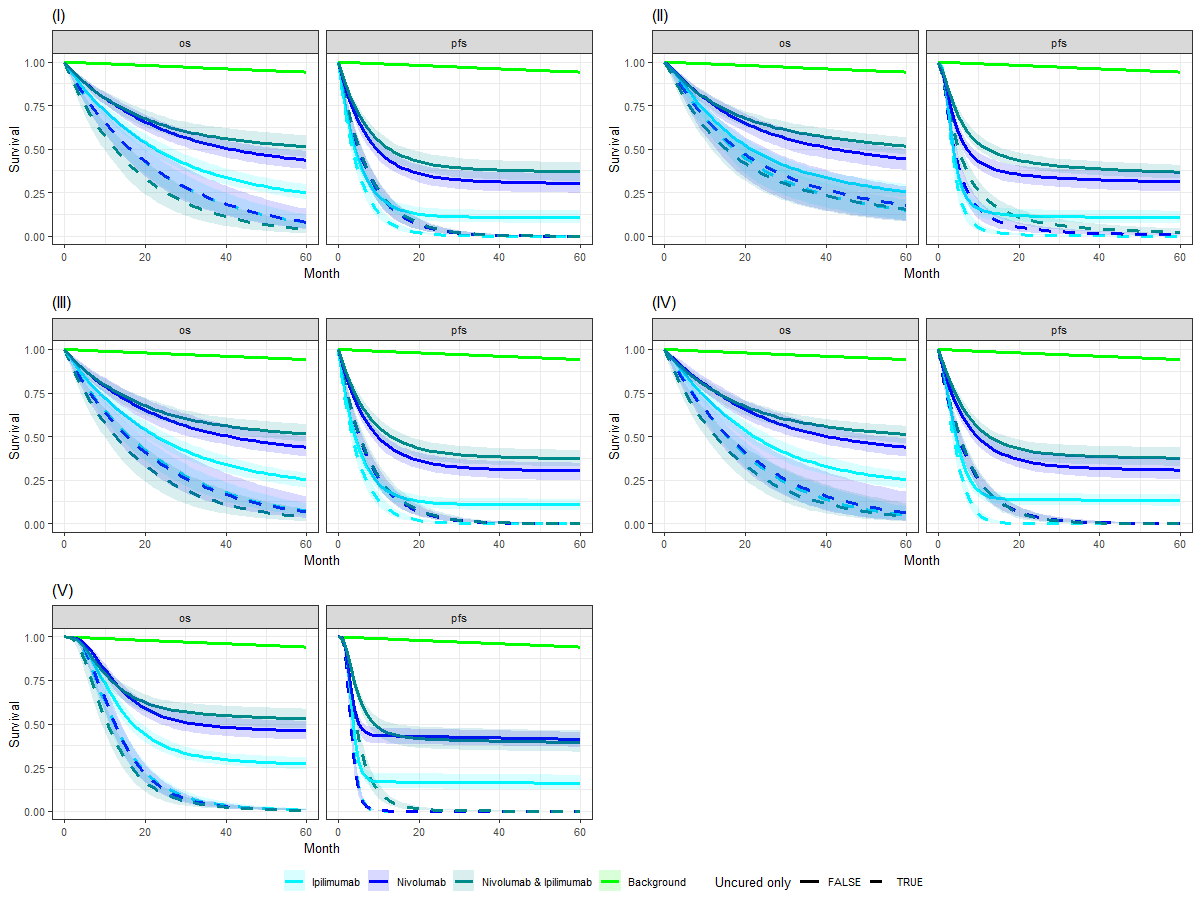
\includegraphics[width=15cm,height=40cm]{../plots/plot_S_samepair_grid_cf_hier_diffuncured} 

}

\caption{\label{fig:S_hier}Posterior survival curves for the mixture cure model for hierarchical OS and PFS models and $ipilimumab$, $nivolumab$ and a combination treatment arm. The green line is cured background. Uncured distributions are I) Exponential  II) Log-logistic III) Gompertz IV) Weibull V) Log-Normal.}\label{fig:unnamed-chunk-7}
\end{figure}

Figure \ref{fig:forest_hier} shows the forest plots of cure fraction
posterior distributions. We see that the values are generally similar
for the Exponential and log-logistic fits. This clearly shows how the
global cure fraction posterior distribution lies partway between the PFS
and OS distributions.

\begin{figure}

{\centering 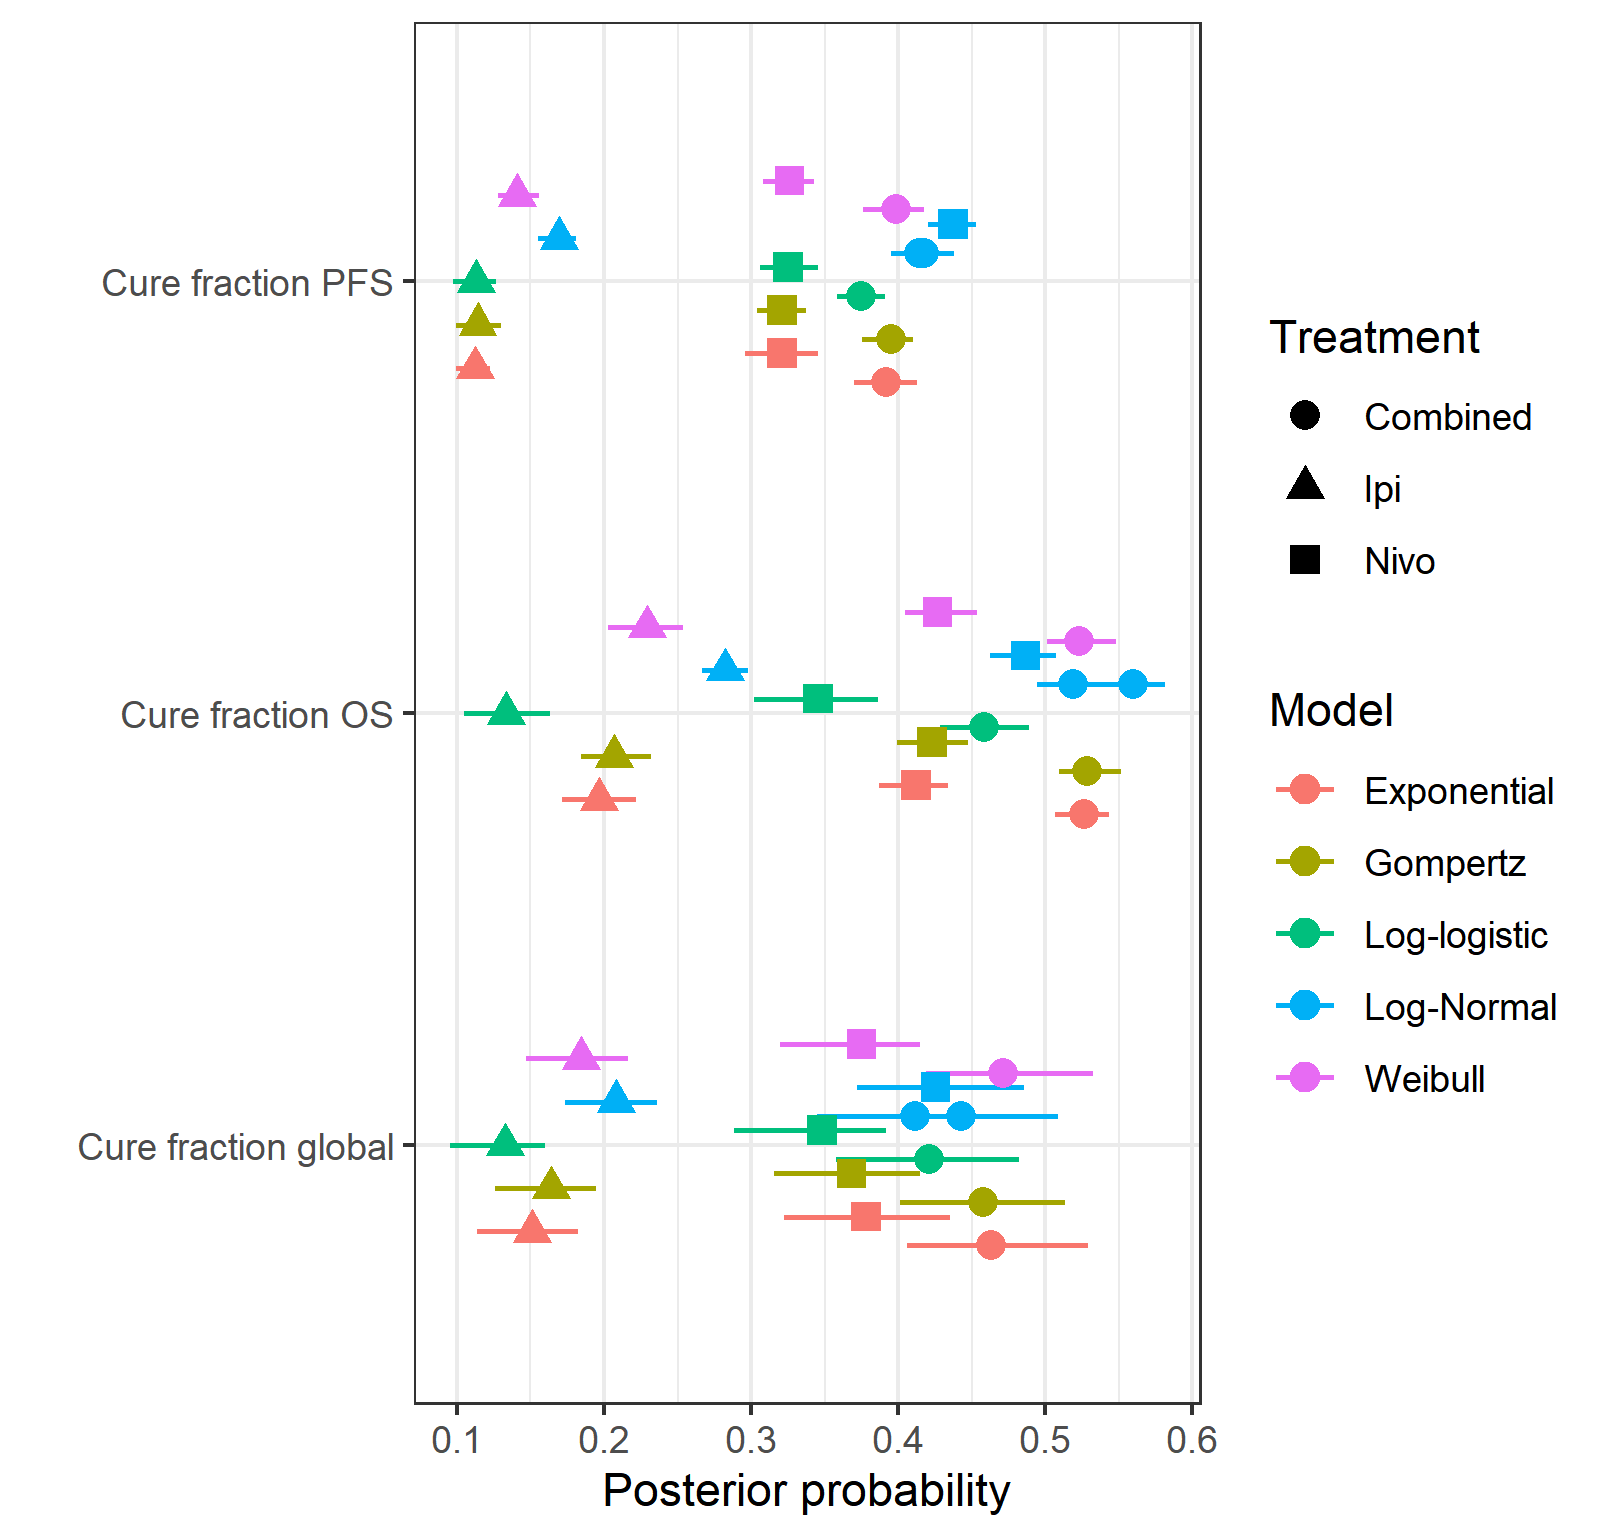
\includegraphics[width=0.6\linewidth]{../plots/cf hier_bg_fixed_forest_plot} 

}

\caption{\label{fig:forest_hier}Forest plot of cure fraction posterior distributions for exchangeable model.}\label{fig:unnamed-chunk-8}
\end{figure}

Table 3 summarises the cure fraction posterior distribution for each
scenario.

\begin{longtable}[]{@{}
  >{\raggedleft\arraybackslash}p{(\columnwidth - 12\tabcolsep) * \real{0.03}}
  >{\raggedright\arraybackslash}p{(\columnwidth - 12\tabcolsep) * \real{0.11}}
  >{\raggedright\arraybackslash}p{(\columnwidth - 12\tabcolsep) * \real{0.11}}
  >{\raggedright\arraybackslash}p{(\columnwidth - 12\tabcolsep) * \real{0.19}}
  >{\raggedright\arraybackslash}p{(\columnwidth - 12\tabcolsep) * \real{0.19}}
  >{\raggedright\arraybackslash}p{(\columnwidth - 12\tabcolsep) * \real{0.19}}
  >{\raggedright\arraybackslash}p{(\columnwidth - 12\tabcolsep) * \real{0.19}}@{}}
\caption{Cure fraction posterior distribution for hierarchical
model.}\tabularnewline
\toprule
\begin{minipage}[b]{\linewidth}\raggedleft
ID
\end{minipage} & \begin{minipage}[b]{\linewidth}\raggedright
OS distn
\end{minipage} & \begin{minipage}[b]{\linewidth}\raggedright
PFS distn
\end{minipage} & \begin{minipage}[b]{\linewidth}\raggedright
Treatment
\end{minipage} & \begin{minipage}[b]{\linewidth}\raggedright
\(cf\) (CrI)
\end{minipage} & \begin{minipage}[b]{\linewidth}\raggedright
\(cf_{OS}\) (CrI)
\end{minipage} & \begin{minipage}[b]{\linewidth}\raggedright
\(cf_{PFS}\) (CrI)
\end{minipage} \\
\midrule
\endfirsthead
\toprule
\begin{minipage}[b]{\linewidth}\raggedleft
ID
\end{minipage} & \begin{minipage}[b]{\linewidth}\raggedright
OS distn
\end{minipage} & \begin{minipage}[b]{\linewidth}\raggedright
PFS distn
\end{minipage} & \begin{minipage}[b]{\linewidth}\raggedright
Treatment
\end{minipage} & \begin{minipage}[b]{\linewidth}\raggedright
\(cf\) (CrI)
\end{minipage} & \begin{minipage}[b]{\linewidth}\raggedright
\(cf_{OS}\) (CrI)
\end{minipage} & \begin{minipage}[b]{\linewidth}\raggedright
\(cf_{PFS}\) (CrI)
\end{minipage} \\
\midrule
\endhead
1 & exp & exp & Ipilimumab & 0.151 (0.068, 0.26) & 0.196 (0.136, 0.255)
& 0.112 (0.079, 0.155) \\
2 & exp & exp & Nivolumab & 0.378 (0.216, 0.557) & 0.412 (0.35, 0.479) &
0.321 (0.262, 0.379) \\
3 & exp & exp & Nivolumab+ipilimumab & 0.463 (0.328, 0.626) & 0.526
(0.452, 0.597) & 0.392 (0.334, 0.448) \\
4 & gompertz & gompertz & Ipilimumab & 0.164 (0.088, 0.275) & 0.207
(0.13, 0.266) & 0.114 (0.079, 0.148) \\
5 & gompertz & gompertz & Nivolumab & 0.368 (0.247, 0.517) & 0.423
(0.358, 0.494) & 0.321 (0.261, 0.369) \\
6 & gompertz & gompertz & Nivolumab+ipilimumab & 0.458 (0.318, 0.612) &
0.529 (0.477, 0.594) & 0.395 (0.346, 0.446) \\
7 & loglogistic & loglogistic & Ipilimumab & 0.133 (0.061, 0.278) &
0.133 (0.054, 0.206) & 0.113 (0.075, 0.152) \\
8 & loglogistic & loglogistic & Nivolumab & 0.348 (0.191, 0.526) & 0.345
(0.231, 0.456) & 0.325 (0.264, 0.382) \\
9 & loglogistic & loglogistic & Nivolumab+ipilimumab & 0.421 (0.266,
0.599) & 0.459 (0.37, 0.535) & 0.375 (0.327, 0.421) \\
10 & lognormal & lognormal & Ipilimumab & 0.208 (0.145, 0.281) & 0.282
(0.246, 0.322) & 0.169 (0.13, 0.219) \\
11 & lognormal & lognormal & Nivolumab & 0.425 (0.286, 0.588) & 0.486
(0.431, 0.546) & 0.437 (0.39, 0.48) \\
12 & lognormal & lognormal & Nivolumab+ipilimumab & 0.442 (0.266, 0.597)
& 0.56 (0.499, 0.621) & 0.417 (0.36, 0.488) \\
13 & weibull & lognormal & Nivolumab+ipilimumab & 0.411 (0.238, 0.596) &
0.519 (0.45, 0.597) & 0.414 (0.347, 0.473) \\
14 & weibull & weibull & Ipilimumab & 0.184 (0.095, 0.29) & 0.229
(0.157, 0.295) & 0.141 (0.107, 0.177) \\
15 & weibull & weibull & Nivolumab & 0.375 (0.242, 0.541) & 0.427
(0.346, 0.494) & 0.326 (0.27, 0.394) \\
16 & weibull & weibull & Nivolumab+ipilimumab & 0.471 (0.328, 0.647) &
0.523 (0.461, 0.58) & 0.399 (0.35, 0.462) \\
\bottomrule
\end{longtable}

Table 4 gives the leave-one-out cross validation WAIC statistics for
each model fit.

\begin{longtable}[]{@{}lllrr@{}}
\caption{Leave-one-out WAIC cross validation statistics for hierarchical
model.}\tabularnewline
\toprule
OS distn & PFS distn & Treatment & Estimate & SE \\
\midrule
\endfirsthead
\toprule
OS distn & PFS distn & Treatment & Estimate & SE \\
\midrule
\endhead
exp & exp & Ipilimumab & 3677.65 & 72.13 \\
exp & exp & Nivolumab & 3359.19 & 91.37 \\
exp & exp & Nivolumab+ipilimumab & 3086.98 & 107.74 \\
gompertz & gompertz & Ipilimumab & 3678.68 & 72.53 \\
gompertz & gompertz & Nivolumab & 3358.96 & 91.59 \\
gompertz & gompertz & Nivolumab+ipilimumab & 3087.62 & 108.05 \\
loglogistic & loglogistic & Ipilimumab & 3536.33 & 78.40 \\
loglogistic & loglogistic & Nivolumab & 3303.47 & 92.04 \\
loglogistic & loglogistic & Nivolumab+ipilimumab & 3067.91 & 106.35 \\
lognormal & lognormal & Ipilimumab & 3122.14 & 111.54 \\
lognormal & lognormal & Nivolumab & 3099.36 & 120.30 \\
lognormal & lognormal & Nivolumab+ipilimumab & 2977.61 & 116.25 \\
weibull & lognormal & Nivolumab+ipilimumab & 3016.47 & 110.29 \\
weibull & weibull & Ipilimumab & 3639.77 & 79.38 \\
weibull & weibull & Nivolumab & 3360.49 & 91.83 \\
weibull & weibull & Nivolumab+ipilimumab & 3088.08 & 108.39 \\
\bottomrule
\end{longtable}

We see that, corresponding to the separate model results, the best
fitting models are for the nivolumab+ipilimumab followed by nivolumab
hierarchical models. Again, the best fitting distributions are lognormal
followed by loglogistic.

In comparison with the separate model fits, the WAIC for the
hierarchical models are mostly better and when the separate model has
smaller estimate it is by a small margin of error.

Table 5 shows the variance partition coefficient (VPC).

\begin{longtable}[]{@{}lllrr@{}}
\caption{Variance partition coefficient (VPC) for hierachical
model.}\tabularnewline
\toprule
OS & PFS & Treatment & vpc\_pfs & vpc\_os \\
\midrule
\endfirsthead
\toprule
OS & PFS & Treatment & vpc\_pfs & vpc\_os \\
\midrule
\endhead
exp & exp & Ipilimumab & 0.813 & 0.784 \\
exp & exp & Nivolumab & 0.876 & 0.877 \\
exp & exp & Nivolumab+ipilimumab & 0.865 & 0.860 \\
gompertz & gompertz & Ipilimumab & 0.781 & 0.743 \\
gompertz & gompertz & Nivolumab & 0.858 & 0.808 \\
gompertz & gompertz & Nivolumab+ipilimumab & 0.899 & 0.888 \\
loglogistic & loglogistic & Ipilimumab & 0.812 & 0.604 \\
loglogistic & loglogistic & Nivolumab & 0.890 & 0.672 \\
loglogistic & loglogistic & Nivolumab+ipilimumab & 0.915 & 0.786 \\
lognormal & lognormal & Ipilimumab & 0.723 & 0.831 \\
lognormal & lognormal & Nivolumab & 0.928 & 0.881 \\
lognormal & lognormal & Nivolumab+ipilimumab & 0.891 & 0.886 \\
weibull & lognormal & Nivolumab+ipilimumab & 0.907 & 0.877 \\
weibull & weibull & Ipilimumab & 0.841 & 0.726 \\
weibull & weibull & Nivolumab & 0.865 & 0.822 \\
weibull & weibull & Nivolumab+ipilimumab & 0.891 & 0.863 \\
\bottomrule
\end{longtable}

It appears the above table that much of the variation is due to between
PFS and OS indicating distinct cure fractions in each. This is to be
expected since there are only two points informing the global cure
fraction distributions.

\hypertarget{sensitivity-analysis-for-background-mortality}{%
\subsection{Sensitivity analysis for background
mortality}\label{sensitivity-analysis-for-background-mortality}}

As a sensitivity analysis, an adjustment factor was applied to the
general population mortality rates to allow for an assessment of the
impact of background hazards on estimation of the cure fraction. A
hazard ratio of 1.63 was applied to the background hazard. This was
obtained from a previous ad-hoc analysis which compared the WHO life
tables with the OS data for complete responders (CR) from CheckMate 067
(N=120, pooled across all 3 arms).

Table 6 summarises the cure fraction posterior distribution for each
scenario.

\begin{longtable}[]{@{}
  >{\raggedleft\arraybackslash}p{(\columnwidth - 12\tabcolsep) * \real{0.03}}
  >{\raggedright\arraybackslash}p{(\columnwidth - 12\tabcolsep) * \real{0.11}}
  >{\raggedright\arraybackslash}p{(\columnwidth - 12\tabcolsep) * \real{0.11}}
  >{\raggedright\arraybackslash}p{(\columnwidth - 12\tabcolsep) * \real{0.19}}
  >{\raggedright\arraybackslash}p{(\columnwidth - 12\tabcolsep) * \real{0.19}}
  >{\raggedright\arraybackslash}p{(\columnwidth - 12\tabcolsep) * \real{0.19}}
  >{\raggedright\arraybackslash}p{(\columnwidth - 12\tabcolsep) * \real{0.19}}@{}}
\caption{Cure fraction posterior distribution for background adjusted
model.}\tabularnewline
\toprule
\begin{minipage}[b]{\linewidth}\raggedleft
ID
\end{minipage} & \begin{minipage}[b]{\linewidth}\raggedright
OS distn
\end{minipage} & \begin{minipage}[b]{\linewidth}\raggedright
PFS distn
\end{minipage} & \begin{minipage}[b]{\linewidth}\raggedright
Treatment
\end{minipage} & \begin{minipage}[b]{\linewidth}\raggedright
\(cf\) (CrI)
\end{minipage} & \begin{minipage}[b]{\linewidth}\raggedright
\(cf_{OS}\) (CrI)
\end{minipage} & \begin{minipage}[b]{\linewidth}\raggedright
\(cf_{PFS}\) (CrI)
\end{minipage} \\
\midrule
\endfirsthead
\toprule
\begin{minipage}[b]{\linewidth}\raggedleft
ID
\end{minipage} & \begin{minipage}[b]{\linewidth}\raggedright
OS distn
\end{minipage} & \begin{minipage}[b]{\linewidth}\raggedright
PFS distn
\end{minipage} & \begin{minipage}[b]{\linewidth}\raggedright
Treatment
\end{minipage} & \begin{minipage}[b]{\linewidth}\raggedright
\(cf\) (CrI)
\end{minipage} & \begin{minipage}[b]{\linewidth}\raggedright
\(cf_{OS}\) (CrI)
\end{minipage} & \begin{minipage}[b]{\linewidth}\raggedright
\(cf_{PFS}\) (CrI)
\end{minipage} \\
\midrule
\endhead
1 & exp & exp & Nivolumab+ipilimumab & 0.45 (0.291, 0.646) & 0.538
(0.473, 0.588) & 0.402 (0.351, 0.457) \\
2 & gompertz & gompertz & Nivolumab+ipilimumab & 0.459 (0.287, 0.616) &
0.541 (0.448, 0.6) & 0.409 (0.349, 0.474) \\
3 & loglogistic & loglogistic & Nivolumab+ipilimumab & 0.433 (0.287,
0.601) & 0.482 (0.374, 0.567) & 0.39 (0.324, 0.444) \\
4 & lognormal & lognormal & Nivolumab+ipilimumab & 0.46 (0.289, 0.648) &
0.583 (0.531, 0.643) & 0.434 (0.381, 0.491) \\
5 & weibull & weibull & Nivolumab+ipilimumab & 0.469 (0.297, 0.62) &
0.546 (0.496, 0.592) & 0.409 (0.354, 0.459) \\
\bottomrule
\end{longtable}

Figure \ref{fig:forest_global_163} shows the equivalent posterior
survival curves to Figures \ref{fig:forest_hier} for the combined
\(ipilimumab\) and \(nivolumab\) treatment and background hazard ratio
adjustment 1.63.

\begin{figure}

{\centering 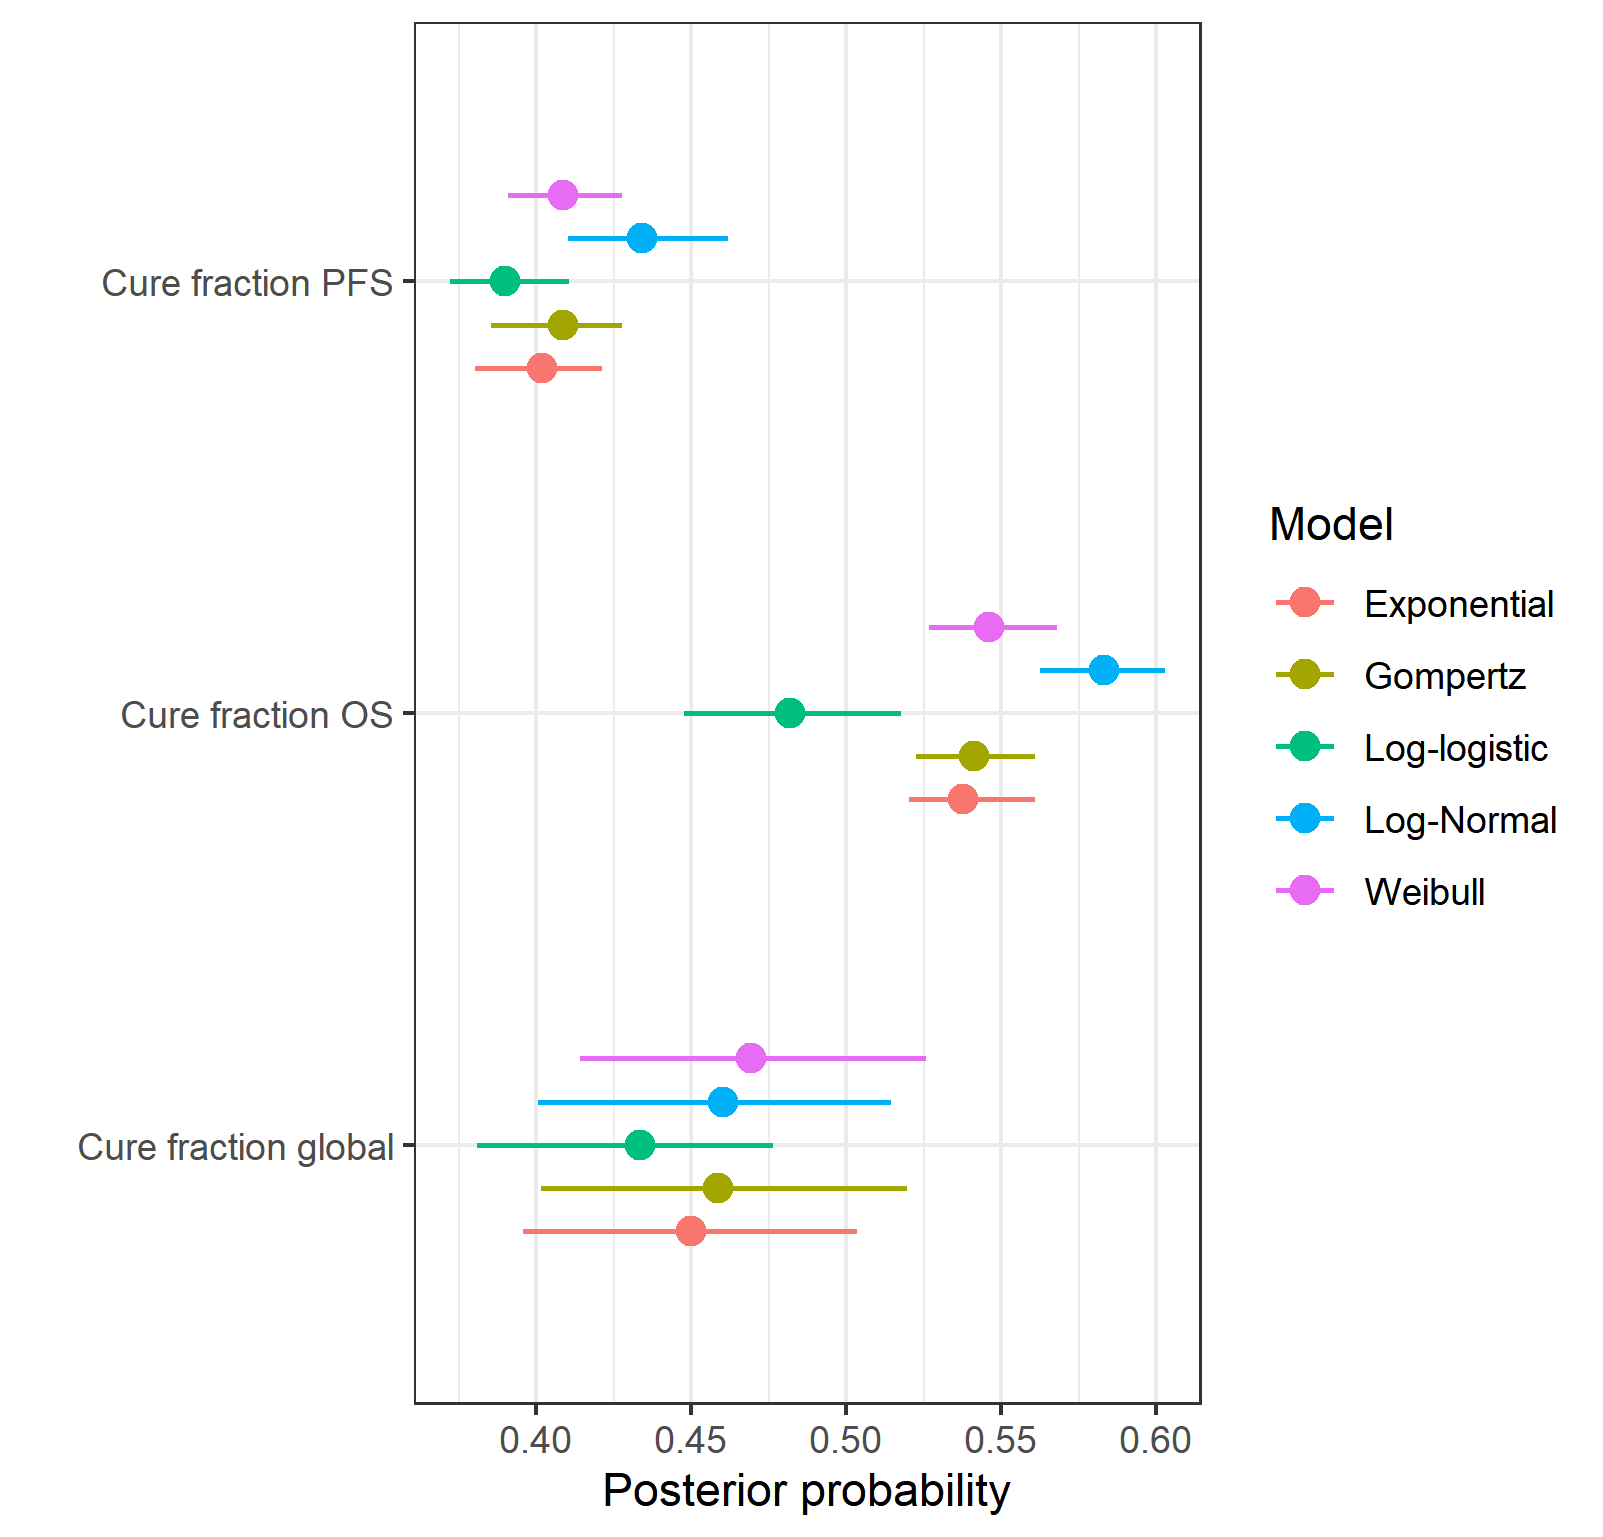
\includegraphics[width=0.6\linewidth]{../plots/cf hier_bg_fixed_hr1.63_forest_plot} 

}

\caption{\label{fig:forest_global_163}Forest plot of cure fraction posterior distributions for dual $ipilimumab$ and $nivolumab$ and background hazard ratio adjustment 1.63.}\label{fig:unnamed-chunk-12}
\end{figure}

\newpage

Table 7 gives the leave-one-out cross validation statistics for each
model fit.

\begin{longtable}[]{@{}lllrr@{}}
\caption{Leave-one-out WAIC cross validation statistics for background
adjusted model.}\tabularnewline
\toprule
OS distn & PFS distn & Treatment & Estimate & SE \\
\midrule
\endfirsthead
\toprule
OS distn & PFS distn & Treatment & Estimate & SE \\
\midrule
\endhead
exp & exp & Nivolumab+ipilimumab & 3096.38 & 106.09 \\
gompertz & gompertz & Nivolumab+ipilimumab & 3097.14 & 106.41 \\
loglogistic & loglogistic & Nivolumab+ipilimumab & 3082.45 & 105.49 \\
lognormal & lognormal & Nivolumab+ipilimumab & 2974.89 & 114.90 \\
weibull & weibull & Nivolumab+ipilimumab & 3098.82 & 107.17 \\
\bottomrule
\end{longtable}

\hypertarget{conclusions}{%
\subsection{Conclusions}\label{conclusions}}

We have presented a Bayesian hierarchical MCM framework which can
alleviate the disparity between individually estimated OS- and PFS-based
LTS rates. It also provides a single shared cure fraction makes sense
both from a HTA perspective, enabling `borrowing of strength' from PFS
for OS and more robust by leveraging all data in the presence of varying
rates of censoring, and from clinical perspective, where we would expect
equivalent LTS proportion across OS and PFS. Further, the parametric
Bayesian models enable extrapolation to lifetime with uncertainty which
are crucial for HTA and QALY estimation.

This work has some current limitations. The presented analysis was
restricted to same distribution combinations for OS and PFS but there is
no reason why any combination could be considered. We also only used
vague uninformative prior distributions in the Bayesian model.

Future planned extensions include the examination of all combinations of
distributions for OS and PFS. We will also incorporate prior clinical
input into analysis and model selection. Because our proposed Bayesian
model produces posterior distributions this can be used as part of a
wider probabilistic decision-theoretic approach. A given model could be
used to evaluate optimal courses of action e.g.~in deciding between
preferable drug treatments. Probabilistic statement can be made not just
about which course of action to take but also the confidence in taking
that action. Commonly, clinical decisions are posed in terms of a
cost-effectiveness analysis. Finally, the development of these methods
and dissemination of easy-to-use, scalable, open-source R package for
external users will be done.

\newpage

\hypertarget{references}{%
\subsection*{References}\label{references}}
\addcontentsline{toc}{subsection}{References}

\hypertarget{refs}{}
\begin{CSLReferences}{1}{0}
\leavevmode\vadjust pre{\hypertarget{ref-Amico2018}{}}%
Amico, Maïlis, and Ingrid Van Keilegom. 2018. {``{Cure Models in
Survival Analysis}.''} \emph{Annual Review of Statistics and Its
Application} 5: 311--42.
\url{https://doi.org/10.1146/annurev-statistics-031017-100101}.

\leavevmode\vadjust pre{\hypertarget{ref-carpenter2017stan}{}}%
Carpenter, Bob, Andrew Gelman, Matthew D Hoffman, Daniel Lee, Ben
Goodrich, Michael Betancourt, Marcus Brubaker, Jiqiang Guo, Peter Li,
and Allen Riddell. 2017. {``Stan: A Probabilistic Programming
Language.''} \emph{Journal of Statistical Software} 76 (1).

\leavevmode\vadjust pre{\hypertarget{ref-McElreath2018}{}}%
McElreath, Richard. 2018. \emph{{Statistical Rethinking: A Bayesian
Course with Examples in R and Stan}}. Chapman and Hall/CRC.

\leavevmode\vadjust pre{\hypertarget{ref-Vehtari2017}{}}%
Vehtari, Aki, Andrew Gelman, and Jonah Gabry. 2017. {``{Practical
Bayesian model evaluation using leave-one-out cross-validation and
WAIC}.''} \emph{Statistics and Computing} 27 (5): 1413--32.
\url{https://doi.org/10.1007/s11222-016-9696-4}.

\leavevmode\vadjust pre{\hypertarget{ref-wholifetables}{}}%
WHO. 2020. {``{Life tables by country}.''}
\url{http://apps.who.int/gho/data/?theme=main\&vid=61160}.

\end{CSLReferences}

\end{document}
